\documentclass[a4paper,12pt, oneside]{book}

% \usepackage{fullpage}
\usepackage[italian]{babel}
\usepackage[utf8]{inputenc}
\usepackage{amssymb}
\usepackage{amsthm}
\usepackage{graphics}
\usepackage{amsfonts}
\usepackage{listings}
\usepackage{amsmath}
\usepackage{amstext}
\usepackage{engrec}
\usepackage{rotating}
\usepackage[safe,extra]{tipa}
\usepackage{showkeys}
\usepackage{multirow}
\usepackage{hyperref}
\usepackage{microtype}
\usepackage{enumerate}
\usepackage{braket}
\usepackage{marginnote}
\usepackage{pgfplots}
\usepackage{cancel}
\usepackage{polynom}
\usepackage{booktabs}
\usepackage{enumitem}
\usepackage{framed}
\usepackage{pdfpages}
\usepackage{pgfplots}
\usepackage[cache=false]{minted}

\usepackage{tikz}\usetikzlibrary{er}\tikzset{multi  attribute /.style={attribute ,double  distance =1.5pt}}\tikzset{derived  attribute /.style={attribute ,dashed}}\tikzset{total /.style={double  distance =1.5pt}}\tikzset{every  entity /.style={draw=orange , fill=orange!20}}\tikzset{every  attribute /.style={draw=MediumPurple1, fill=MediumPurple1!20}}\tikzset{every  relationship /.style={draw=Chartreuse2, fill=Chartreuse2!20}}\newcommand{\key}[1]{\underline{#1}}

\usepackage{fancyhdr}
\pagestyle{fancy}
\fancyhead[LE,RO]{\slshape \rightmark}
\fancyhead[LO,RE]{\slshape \leftmark}
\fancyfoot[C]{\thepage}



\title{Ricerca Operativa e Pianificazione delle Risorse}
\author{UniShare\\\\Davide Cozzi\\\href{https://t.me/dlcgold}{@dlcgold}\\\\Gabriele De Rosa\\\href{https://t.me/derogab}{@derogab} \\\\Federica Di Lauro\\\href{https://t.me/f_dila}{@f\textunderscore dila}}
\date{}

\pgfplotsset{compat=1.13}
\begin{document}
\maketitle

\definecolor{shadecolor}{gray}{0.80}
\setlist{leftmargin = 2cm}
\newtheorem{teorema}{Teorema}
\newtheorem{definizione}{Definizione}
\newtheorem{esempio}{Esempio}
\newtheorem{corollario}{Corollario}
\newtheorem{lemma}{Lemma}
\newtheorem{osservazione}{Osservazione}
\newtheorem{nota}{Nota}
\newtheorem{esercizio}{Esercizio}
\tableofcontents
\renewcommand{\chaptermark}[1]{%
  \markboth{\chaptername
    \ \thechapter.\ #1}{}}
\renewcommand{\sectionmark}[1]{\markright{\thesection.\ #1}}
\chapter{Introduzione}
\textbf{Questi appunti sono presi a lezione. Per quanto sia stata
  fatta una revisione è altamente probabile (praticamente certo)
  che possano contenere errori, sia di stampa che di vero e proprio
  contenuto. Per eventuali proposte di correzione effettuare una
  pull request. Link: } \url{https://github.com/dlcgold/Appunti}.\\
\textbf{Grazie mille e buono studio!}
\chapter{Introduzione alla Ricerca Operativa}
La\textbf{ Ricerca Operativa} è essenziale nel \textit{problem
  solving} e nell'ambito del \textit{decision making}.
Sostanzialmente quindi si studia l'ottimizzazione, massimizzando le
performances, l'accuratezza dei costi etc$\ldots$ per raggiungere un
obiettivo. \\ \textit{Sulle slides ci sono vari esempi introduttivi di
  vita reale}\\
Un altro problema studiato dalla riceca operativa sono le previsioni,
mediante algoritmi predittivi che studiano i \textit{pesi} delle
osservazioni (cosa utile nel \textbf{Machine Learning} in quanto sono
un uso di base delle \textbf{Reti Neurali}, \textit{vari esempi
  introduttivi sulle slides}).\\
\textbf{La ricerca operativa si occupa di formalizzare un problema in
  un modello matematico e calcolare una soluzione ottimo o
  approssimata}. Essa costituisce un approccio scientifico alla
risoluzione di problemi complessi da ricondurre alla matematica
applicata. È utile in ambiti economici, logistici, di progettazione di
servizi e di sistemi di trasporto e, ovviamente, nelle tecnologie.
\textit{È la branca della matematica più applicata}.\\
Il \textit{primo passo} consiste nel costruire un modello traducendo il
problema reale in linguaggio anturale in un linguaggio matematico, che
non è ambiguo. Il \textit{secondo passo} consiste nella costruzione delle
soluzioni del modello tramite algoritmi e programmi di calcolo. Il
\textit{terzo passo}, ovvero l'ultimo, è l'interpretazione e la
valutazione delle soluzioni del modello rispetto a quelle del problema
reale.\\
La ricerca operativa ha origini nel 1800 in un ambiente puramente
matematico. È stata resa ``\textit{algoritmica}'' con la Macchina di
Turing. \textbf{La ricerca operativa usa anche tecniche numeriche e
  non solo analitiche}.\\
Negli ultimi hanno si sono sviluppati, mediante il concetto di
\textbf{gradiente}, nuovi algoritmi per il \textbf{deep network}.\\
\section{Modelli nella R.O.}
\begin{definizione}
  Data una funzione $f:\mathbb{R} \to mathbb{R}$ e $X\subseteq
  \mathbb{R}^n$ un \textbf{problema di ottimizzazione} può esssere
  formulato come:
  \[opt\,\,f(x)\,\,s.t. \,\,x\in X\]
  dove con $opt={\min, \max}$ indendiamo che opt può essere o min o max,
  portando ad un problema di minimizzazione con $\min\,f(x)$ o di
  massimizzazione $\max\,f(x)$. \\
  $f(x)$ è detta \textbf{funzione obiettivo} e vale che:
  \[max[f(x):\,x\in X] = -min[-f(x):\,x\in X]\]
  Inoltre $x\subseteq\mathbb{R}^n$ è \textbf{l'insieme delle soluzioni
    ottenibili} o anche \textbf{regione ammissibile}.\\
  Infine $x\in X$ rappresenta il \textbf{vettore delle variabili
    decisionali} e si tratta di variabili numeriche i cui valori
  rappresentano la soluzione del problema. \\
  \textbf{Si capisce che essendo in $\mathbb{R}$ si hanno infinite
    soluzioni}.\\
  % aggiungere fine definizione

  Se $X=\mathbb{R}^n$ si ha un'\textbf{ottimizzazione non vincolata}, altrimenti,
  $x\subset \mathbb{R}$ si ha un'\textbf{ottimizzazione vincolata}, dove la
  ricerca dei punti di ottimo della funzione obiettivo è fatta su un
  sottoinsieme proprio dello spazio di definizione tenendo però conto
  dei vincoli. Se ho una funzione obiettivo lineare non si può avere
  un'ottimizzazione non vincolata (non saprei cercare massimi e minimi
  senza vincoli).\\
  Abbiamo poi l'\textbf{ottimizzazione intera o a numeri interi}
  se $x\in \mathbb{Z}^n$ e si possono avere ottimizzazioni miste se si
  hanno interi e reali. Si ha anche l'\textbf{ottimizzazione binaria}
  quando si hanno due vie decisionali. \\
  \textbf{Se non specificato si intende $X\subseteq\mathbb{R}}$.
\end{definizione}
\begin{definizione}
  Quando l'insieme $X$ delle soluzioni ammissibili di un problema di
  ottimizzazione è espresso in un sistema di equazioni o disequazioni si
  parla di \textbf{problema di programmazione matematica (PM)}.\\
  Come vincolo si ha un'espressione $g_i(x)\{\leq, =, \geq\} 0$
  ($g_i\geq 0$ etc $\ldots$) e con
  $g_i:X\to \mathbb{R}$ che è una generica funzione che lega due
  variabili. \\
  \textbf{Si possono avere più vincoli ma si ha sempre l'uguale in ogni
    vincolo per permettere il funzionamento degli algoritmi}.\\
  La regione ammissibile è $X\subseteq\mathbb{R}^n$ che è l'intersezione
  di tutti i vincoli del problema
  \[X=\{x\in\mathbb{R}^n|\, g_i(x)\{\leq, 0, \geq\}\]
  % termina definizione
\end{definizione}
\begin{esempio}
  abbiamo la funzione obiettivo
  \[\min_{x,y}(x^2+y^2)\]
  con i 3 vincoli:
  \[x+y \leq 3\]
  \[x\geq 0\]
  \[y\geq 0\]
  la regione ammissibile è:
  \[\{x\in\mathbb{R}^2|\,x+y \leq 3,\,\,x\geq 0,\,\,y\geq 0\}\]
  % inserire grafico
\end{esempio}
Si possono avere problemi con regione non ammissibile, ovvero con
$X=\emptyset$, che implica che il problema è mal posto oppure bisogna
abbassare qualche vincolo. Si può avere un problema illimitato con:
\[\forall c \in \mathbb{R}\exists x_c\in X:f(x_c)\leq c\,\, se\,\,
  opt = min\]
\[\forall c \in \mathbb{R}\exists x_c\in X:f(x_c)\geq c\,\, se\,\,
  opt = max\]
Infine si può avere una sola soluzione ottima o più (anche infinite)
soluzioni ottime
% finire frase
\begin{esempio}
  abbiamo la funzione obiettivo
  \[\min_{x,y}(x^2+y^2)\]
  con i 3 vincoli:
  \[x+y \leq -1\]
  \[x\geq 0\]
  \[y\geq 0\]
  Non ha soluzione (è matematicamente impossibile) e il problema
  non è ammissibile
\end{esempio}
\begin{esempio}
  abbiamo la funzione obiettivo
  \[\max_{x,y}(x^2+y^2)\]
  con i 2 vincoli:
  \[x\geq 0\]
  \[y\geq 0\]
  Ha come soluzione infinito
\end{esempio}
\begin{esempio}
  abbiamo la funzione obiettivo
  \[\max_{x,y,z}(z)\]
  con i 4 vincoli:
  \[x+y+z = 2\]
  \[0\leq x \leq 1\]
  \[0\leq y \leq 1\]
  \[0\leq z \leq 1\]
  Ha infinite soluzioni (tutte le soluzioni con $z=1$ e $x+y=1$, in quanto cerco
  il max di z e come ultio vincolo ho che al massimo è 1)
  % aggiungere grafico
\end{esempio}
La risoluzione di un problema di Programmazione matematica consiste
nel trovare una soluzione ammissibile che sia un \textbf{ottimo
  globale} ovvero un vettore $^*\in X$ tale che:
\[f(x^*)\leq f(x)\,\,\forall x\in X\,\,se\,\,opt=\min\]
\[f(x^*)\geq f(x)\,\,\forall x\in X\,\,se\,\,opt=\max\]
Quando il problema è molto difficile da risolvere possiamo
accontentarci di un ottimo locale, vale a dire un $\hat{x}\in X$ tale
che, fissato un $\varepsilon > 0$ opportuno si ha che (per problemi di
minimo e massimo):
\[f(\hat{x})\leq f(x)\,\,\forall x\in X:\,\||x-\hat{x}||\leq
  \varepsilon\,\,se\,\,opt=\min\]
\[f(\hat{x})\geq f(x)\,\,\forall x\in X:\,\||x-\hat{x}||\leq \varepsilon\,\,se\,\,opt=\max\]
Un problema di ottimizzazione può avere più ottimi locali e globali e
i punti di ottimo globale sono anche di ottimo locale.
\begin{center}
  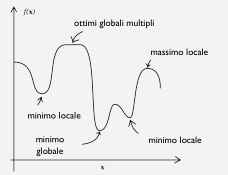
\includegraphics[scale = 1.3]{img/opt.png}
\end{center}
\newpage
\begin{esempio}
  abbiamo la funzione obiettivo:
  \[\min_{x,y}((x-0.2)^2+y^2)\]
  con i 3 vincoli:
  \[x+y \leq 1\]
  \[x\geq 0\]
  \[y\geq 0\]
  In viola si ha la funzione obiettivo tridimensionale e convessa
  e in azzurro la regione ammissibile
  \begin{center}
    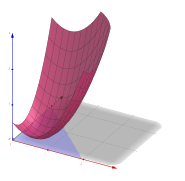
\includegraphics[scale = 1.3]{img/optes.png}
  \end{center}
  si ha solo un minimo globale.
  Si possono usare le \textbf{curve di livello} che sono le linee
  parallele al piano (approfondire!!!!).\\
  In generale si useranno tecniche numeriche anche se si ha che
  \textbf{una funzione convessa ha un solo minimo globale}
\end{esempio}
\newpage
\begin{esempio}
  abbiamo la funzione obiettivo:
  \[\min_{x}(0.2x^2+(1-\cos(\pi x)))\]
  con i 2 vincoli:
  \[x\geq 5\]
  \[y\geq 0\]
  e si ha il seguente grafico:
  \begin{center}
    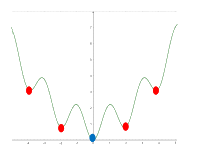
\includegraphics[scale = 1.3]{img/optes2.png}
  \end{center}
  si ha il coseno quindi si ha una funzione nè concava nè convessa
  si ha quindi un ottimo globale e 4 locali
\end{esempio}
Si ha:
\begin{itemize}
  \item \textbf{programmazione lineare (PL)}, con obiettivo e vincoli
  lineari:
  \[opt\,f(x)=c^T x\]
  \[X=\{x\in\mathbb{R}^n:\, g_i(x)\{\leq, =, \geq\}0,\,\,
    i=1,\ldotsm\,\, g_i(x)=a_i^T x-b_i\}\]
  \item \textbf{programmazione lineare intera (PLI)}, con obiettivo e
  vincoli lineari interi:
  \[opt\,f(x)=c^T x\]
  \[X=\{x\in\mathbb{Z}^n:\, g_i(x)\{\leq, =, \geq\}0,\,\,
    i=1,\ldotsm\,\, g_i(x)=a_i^T x-b_i\}\]
  \item \textbf{programmazione non lineare (PNL)}, con obiettivo e
  vincoli $g_i(x)$ non lineari:
  \[opt\,f(x)\]
  \[X=\{x\in\mathbb{R}^n:\, g_i(x)\{\leq, =, \geq\}0,\,\,
    i=1,\ldotsm\,\, g_i(x)=a_i^T x-b_i\}\]
\end{itemize}
\begin{esempio}
  abbiamo la funzione obiettivo:
  \[\min_{x,y}(x^2+y^2)\]
  con i 3 vincoli:
  \[x+y\leq 1\]
  \[x\geq 0\]
  \[y\geq 0\]
  non è lineare in quanto x e y sono al quadrato e quindi non lineare
\end{esempio}
\begin{esempio}
  abbiamo la funzione obiettivo:
  \[\min_{x,y}(x+y)\]
  con i 2 vincoli:
  \[x^2-1\geq 0\]
  \[y\geq 0\]
  non è lineare in quanto ho un vincolo al quadrato e quindi non
  lineare 
\end{esempio}
\begin{esempio}
  abbiamo la funzione obiettivo:
  \[\min_{x,y}(x+4y)\]
  con i 4 vincoli:
  \[x+y=3\]
  \[x^2-1\geq 0\]
  \[x\geq 0\]
  \[y\geq 0\]
  non è lineare in quanto ho un vincolo al quadrato e quindi non
  lineare ma posso renderlo lineare in quanto $x^2-1=(x-1)(x+1)$ ma
  $x+1$ è sempre positivo quindi posso ammorbidire il vincolo
  rendendo il problema lineare
\end{esempio}
\begin{esempio}
  \begin{center}
    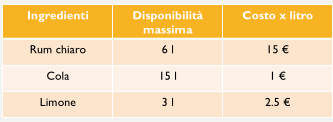
\includegraphics[scale = 0.7]{img/cub.png}
  \end{center}
  Le dosi ideali sono: almeno il 25\% di rum (R) chiaro e il 50\% di
  Cola (C) e non più del 10\% di limone (L) e voglio 10L di cubalibre. Abbiamo quindi, per logica:
  \[R\geq 0\]
  \[C\geq 0\]
  \[L\geq 0\]
  \[R\leq 6\]
  \[C\leq 15\]
  \[L\leq 3\]
  quindi:
  \[0\leq R\leq 6\]
  \[0\leq C\leq 15\]
  \[0\leq L\leq 3\]
  inoltre:
  \[R+C+L\geq 10\]
  che è:
  \[R+C+L -10\geq 0 = \left[
      \begin{matrix}
        1 & 1 & 1
      \end{matrix}
    \right]\left[
      \begin{matrix}
        R \\
        C \\
        L
      \end{matrix}
    \right] -10 \geq 0\]
  quindi:
  \[a_1^T= \left[
      \begin{matrix}
        1 & 1 & 1
      \end{matrix}
    \right], \,x =\left[
      \begin{matrix}
        R \\
        C \\
        L
      \end{matrix}
    \right],\, b_1=10 \]
  Cosa vuol dire almeno il 25\% di rum chiaro?
  \[R \geq 0.25 \cdot (R + C + L)\]
  Cosa vuol dire almeno il 5o\% di cola?
  \[R \geq 0.5 \cdot (R + C + L)\]
  Cosa vuol dire almeno il 25\% di limone?
  \[R \geq 0.1\cdot (R + C + L)\]
  che sono vincoli lineari.\\
  quindi il costo è:
  \[\min_{R,C,L}(15R+C+2.5L)\]
  che è una funzione obiettivo lineare.\
  Osserviamo che la funzione obiettivo può essere scritta anche nella
  seguente forma compatta:
  \[\min c^tx,\,\con\,\,c^t=\left[
      \begin{matrix}
        15 & 1 & 2.5
      \end{matrix}
    \right]\,\,e\,\, x =\left[
      \begin{matrix}
        R \\
        C \\
        L
      \end{matrix}
    \right] \]
  Ora riscriviamo in forma matriciale:
  \[\min cx\]
  \[Ax\geq b\]
  \[x\geq 0\]
  con:
  \[c=\left[
      \begin{matrix}
        15 & 1 & 2.5
      \end{matrix}
    \right]\]
  \[x =\left[
      \begin{matrix}
        R \\
        C \\
        L
      \end{matrix}
    \right]\]
  la prima riga sarà $R+C+L\geq 10$\\
  la seconda sarà $R\geq 0.25\cdot (R+C+L) \geq 0 \to
  (1-0.25)R-0.25R-0.25L$\\
  la terza sarà $C\geq 0.5\cdot (R+C+L) \geq 0 \to
  -0.5R + (1-0.5)C-0.5L$\\
  la quarta sarà $L\geq 0.1\cdot (R+C+L) \geq 0 \to
  -0.1R -0.25C +0.9(1-0.1)L$\\
  la quinta sarà $0 \leq R \leq 6 \to -R \geq -6$\\
  la sesta sarà $0 \leq C \leq 15 \to -C \geq -6$\\
  la settima sarà $0 \leq L \leq 3 \to -L \geq -6$\\
  e quindi:
  \[Ax=\left[
      \begin{matrix}
        1 & 1 & 1 \\
        0.75 & -0.25 & -0.25 \\
        -0.5 & 0.5 & -.5 \\
        0.1 & 0.1 & -0.9 \\
        -1 & 0 & 0 \\
        0 & -1 & 0 \\
        0 & 0 & -1
      \end{matrix}
    \right]
    \left[
      \begin{matrix}
        R \\
        C \\
        L
      \end{matrix}
    \right] \geq
    \left[
      \begin{matrix}
        10 \\
        0 \\
        0 \\
        0 \\
        -6 \\
        -15 \\
        -3 
      \end{matrix}
    \right]\]
\end{esempio}

\begin{esempio}
  Si ha che:
  \begin{center}
    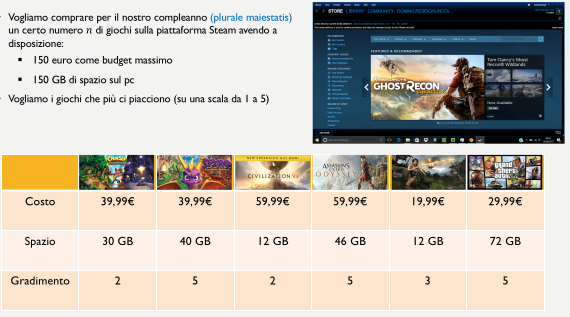
\includegraphics[scale = 0.7]{img/steam.png}
  \end{center}
  Il comprare o no un videogioco può essere modellizzato per mezzo
  di variabili decisionali binarie associate ad ogni gioco usando
  variabili binarie:
  \[x_i\in\{0,1\}\,i=1,\ldots n\]
  con $x_i=1$ si compra con $x_i=0$ no.\\
  Non superare il budget massimo di 100 euro può essere espresso
  dalla seguente relazione:
  \[39,99 \cdot x_1 + 39,99 \cdot x_2 + 59,99 \cdot x_3 + 59,99 \cdot
    x_5 + 19,99 \cdot x_5+ 29,99 \cdot x_6 ≤ 150\]
  Non superare la memoria massima può essere espresso dalla seguente
  relazione:
  \[30 \cdot x_1 + 40 \cdot x_2 + 12 \cdot x_3 + 46 \cdot
    x_5 + 12 \cdot x_5+ 70 \cdot x_6 ≤ 150\]
  e sono vincoli lineari.\\
  Volere i giochi che più ci piacciono si esprime nel seguente modo:
  \[\max(2\cdot x_1+5\cdot x_2+2\cdot x_3+5\cdot x_4+3\cdot x_5+5\cdot x_6)\]
  che è una funzione obiettivo lineare.\\
  Volere i giochi che più ci piacciono, avendo 200 euro di budget e
  100GB si spazio corrisponde a:
  \[\max(2\cdot x_1+5\cdot x_2+2\cdot x_3+5\cdot x_4+3\cdot x_5+5\cdot x_6)\]
  \textbf{Si tratta, quindi, di un problema di programmazione lineare a
    variabili binarie, che sono un caso particolare di variabili
    intere}.\\
  \textbf{\textit{Un modello di ottimizzazione di questo tipo prende
      il nome di Problema dello zaino (Knapsack)}}
\end{esempio}
\textbf{altri esempi sulle slide}
\begin{esempio}
Partendo dai dati di vendita di avatar capire se Endgame supererà gli
incassi di avaatar, sapendo gli incassi dei primi giorni.\\
Vogliamo costruire una retta di regressione lineare che interpoli i
dati:
\[y=ax+b,\,\,a,b\in\mathbb{R}\]
Bisogna calcolare la retta di regressione corrisponde al seguente problema di
ottimizzazione non vincolata:
\[\min_{a,b}\left[\frac{1}{2}\sum_{i=1}^n (y_i-ax_i-b)^2\right]\]
e quindi si ha funzione obiettivo non-lineare con $a,b$ variabili
continue. Cerco quindi la retta di regressione partendo dai primi dati
e ipotizzo una previsione e cerco $a$ e $b$
:
\begin{center}
  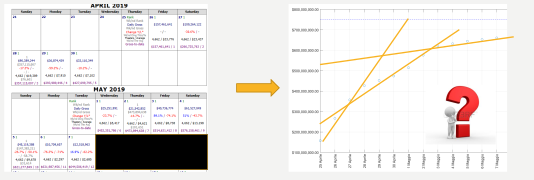
\includegraphics[scale = 0.9]{img/prev.png}
\end{center}

\begin{center}
  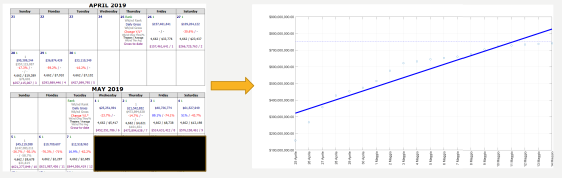
\includegraphics[scale = 0.9]{img/prev2.png}
\end{center}
\textbf{Questo è un problema di ottimizzazione non vincolata e non lineare}
\end{esempio}
\textbf{altri esempi sulle slide}
\end{document}